\chapter{Linear and Angular Momentum Principles}

\section{Single Particle}

\begin{figure}[H]
  \begin{center}
    \begin{tikzpicture}[>={Stealth[width=2mm,length=3mm]}]
      \node[circle, fill=black, inner sep=0pt,minimum size=4pt, label=$m$] (m) at (0,0){};
      \node[circle, fill=black, inner sep=0pt,minimum size=4pt, label=$O$] (O) at (-4,-3){};
      \node[circle, fill=black, inner sep=0pt,minimum size=4pt, label=$B$] (B) at (-2,-4){};
      \draw [->] (-4,-3)--(0,0) node[pos=0.5] {$\underline{r}_{Om}$};
      \draw [->] (0,0)--(2,1) node[pos=0.5] {$\underline{F}$};
      \draw [->] (0,0)--(1,-1) node[pos=0.5] {$\underline{v}$};
      \draw [->] (-4,-3)--(-2,-4) node[pos=0.5] {$\underline{r}_{OB}$};
      \draw [->] (-2,-4)--(0,0) node[pos=0.5] {$\underline{r}_{Bm}$};
    \end{tikzpicture}
    \caption{\fontsize{10pt}{10pt}\selectfont\textbf{Point mass $m$ under action of force $\underline{f}$. Point $O$ is fixed in inertial space, and point $B$ is a general point, not necessarily fixed in inertial space.}}
  \end{center}
\end{figure}

\begin{empheq}[box=\fboxTwo]{alignat*=3}
  &\mbox{\textbf{Linear momentum:}}
  &\hspace{0.5in} \underline{p}=m\underline{v}
\end{empheq}

\begin{empheq}[box=\fboxTwo]{alignat*=3}
  &\mbox{\textbf{Linear momentum principle:}}
  &\hspace{0.5in} \underline{f}=\frac{d\underline{p}}{dt}
\end{empheq}

\begin{empheq}[box=\fboxTwo]{alignat*=3}
  &\mbox{\textbf{Torque about point} $O$:}
  &\hspace{0.5in} \tau_{O}=\underline{r}_{Om}\times\underline{f}
\end{empheq}

\begin{empheq}[box=\fboxTwo]{alignat*=3}
  &\mbox{\textbf{Moment of momentum about point} $O$:}
  &\hspace{0.5in} h_{O}=\underline{r}_{Om}\times\underline{p}
\end{empheq}

differentiate expression for $h_{O}$

\begin{equation*}
  \frac{d}{dt}\underline{h}_{O}=\frac{d}{dt}\underline{r}_{Om}\times\underline{p}+\underline{r}_{Om}\times\frac{d}{dt}\underline{p}
\end{equation*}

but

\begin{equation*}
  \frac{d}{dt}\underline{r}_{Om}=\underline{v}
\end{equation*}

and since $\underline{p}=m\underline{v}$ the cross product $\frac{d}{dt}\underline{r}_{Om}\times\underline{p}=0$ and so

\begin{equation*}
  \frac{d}{dt}\underline{h}_{O}=\underline{r}_{Om}\times\frac{d}{dt}\underline{p}
\end{equation*}

and substituting the linear momentum principle $\frac{d\underline{p}}{dt}=\underline{f}$ this gives

\begin{equation*}
  \frac{d}{dt}\underline{h}_{O}=\underline{r}_{Om}\times\underline{f}
\end{equation*}

But the right hand side is just the torque about point $O$, so we have

\begin{empheq}[box=\fboxTwo]{alignat*=3}
  &\mbox{\textbf{Angular momentum principle of particle about point} $O$:}
  &\hspace{0.5in} \underline{\tau}_{O}=\frac{d}{dt}\underline{h}_{O}
\end{empheq}

About a general point $B$ the torque and moment of momentum can be expressed as

\begin{equation*}
  \begin{split}
    \underline{\tau}_{B}&=\underline{r}_{Bm}\times\underline{f} \\
    \underline{h}_{B}&=\underline{r}_{Bm}\times\underline{p}
  \end{split}
\end{equation*}

Using $\underline{r}_{Bm}=\underline{r}_{Om}-\underline{r}_{OB}$ and substituting in we have

\begin{equation*}
  \begin{split}
    \underline{\tau}_{B}
    &=(\underline{r}_{Om}-\underline{r}_{OB})\times\underline{f} \\
    &=\underline{r}_{Om}\times\underline{f}-\underline{r}_{OB}\times\underline{f} \\
    &=\underline{\tau}_{O}-\underline{R}_{OB}\times\underline{f}
  \end{split}
\end{equation*}

\begin{empheq}[box=\fboxTwo]{alignat*=3}
  &\mbox{\textbf{Torque on particle about general point} $B$:}
  &\hspace{0.5in} \underline{\tau}_{B}=\underline{\tau}_{O}-\underline{r}_{OB}\times\underline{f}
\end{empheq}

and

\begin{equation*}
  \begin{split}
    \underline{h}_{B}&=(\underline{r}_{Om}-\underline{r}_{OB})\times\underline{p} \\
    &=\underline{r}_{Om}\times\underline{p}-\underline{r}_{OB}\times\underline{p} \\
    &=\underline{h}_{O}-\underline{r}_{OB}\times\underline{p}
  \end{split}
\end{equation*}

\begin{empheq}[box=\fboxTwo]{alignat*=3}
  &\mbox{\textbf{Moment of momentum of particle about gen.\ point} $B$:}
  &\hspace{0.5in} \underline{h}_{B}=\underline{h}_{O}-\underline{r}_{OB}\times\underline{p}
\end{empheq}

Evaluate the following

\begin{equation*}
  \begin{split}
    \frac{d}{dt}\underline{h}_{B}&=\frac{d}{dt}\underline{h}_{O}-\frac{d}{dt}\underline{r}_{OB}\times\underline{p}-\underline{r}_{OB}\times\frac{d}{dt}\underline{p} \\
    &=\underline{\tau}_{O}-\underline{v}_{B}\times\underline{p}-\underline{r}_{OB}\times\underline{f}
  \end{split}
\end{equation*}

From above we have $\underline{r}_{OB}\times\underline{f}=\underline{\tau}_{O}-\underline{\tau}_{B}$ and so we can write

\begin{equation*}
  \begin{split}
    \frac{d}{dt}\underline{h}_{B}&=\underline{\tau}_{O}-\underline{v}_{B}\times\underline{p}-\underline{\tau}_{O}+\underline{\tau}_{B} \\
    &=-\underline{v}_{B}\times\underline{p}+\underline{\tau}_{B}
  \end{split}
\end{equation*}

solving for $\underline{\tau}_{B}$ this gives

\begin{empheq}[box=\fboxTwo]{alignat*=3}
  &\mbox{\textbf{Angular momentum principle of particle about gen.\ point} $B$:}
  &\hspace{0.5in} \underline{\tau}_{B}=\frac{d}{dt}\underline{h}_{B}+\underline{v}_{B}\times\underline{p}
\end{empheq}

\section{General System (System of Particles)}

\begin{figure}[H]
  \begin{center}
    \begin{tikzpicture}[>={Stealth[width=2mm,length=3mm]}]
      \pgfmathsetseed{3}
      \draw [fill=yellow!70!black] plot [smooth cycle, samples=8,domain={1:8}] (\x*360/8+5*rnd:1.0cm+1.0cm*rnd) {};
      \node[circle, fill=black, inner sep=0pt,minimum size=4pt, label=$i$] (m) at (0,0){};
      \node[circle, fill=black, inner sep=0pt,minimum size=4pt, label=$O$] (O) at (-4,-3){};
      \node[circle, fill=black, inner sep=0pt,minimum size=4pt, label=$B$] (B) at (-2,-4){};
      \draw [->] (-4,-3)--(0,0) node[pos=0.5, above] {$\underline{r}_{Oi}$};
      \draw [->] (0,0)--(1,-1) node[pos=0.5, above] {$\underline{p}_{i}$};
      \draw [->] (-4,-3)--(-2,-4) node[pos=0.5, above] {$\underline{r}_{OB}$};
      \draw [->] (-2,-4)--(0,0) node[pos=0.5, above] {$\underline{r}_{Bi}$};
    \end{tikzpicture}
    \caption{\fontsize{10pt}{10pt}\selectfont\textbf{General system which is made up of many masses $m_{i}$, with total mass $M$. There are forces $\underline{f}_{i}$ acting on the $i$ particles. Point $O$ is fixed in inertial space, and point $B$ is a general point, not necessarily fixed in inertial space.}}
  \end{center}
\end{figure}

\begin{empheq}[box=\fboxTwo]{alignat*=3}
  &\mbox{\textbf{Linear momentum principle for general system:}}
  &\hspace{0.5in} \underline{F}^{\text{ext}}=\frac{d}{dt}\underline{P}
\end{empheq}

\begin{equation*}
  \underline{H}_{O}=[I]_{O}\omega
\end{equation*}

\begin{empheq}[box=\fboxTwo]{alignat*=3}
  &\mbox{\textbf{Angular momentum principle of general system about point} $O$:}
  &\hspace{0.5in} \underline{\tau}_{O}^{\text{ext}}=\frac{d}{dt}\underline{H}_{O}
\end{empheq}

\begin{empheq}[box=\fboxTwo]{alignat*=3}
  &\mbox{\textbf{Moment of momentum of general system about point} $B$:}
  &\hspace{0.5in} \underline{H}_{B}=\underline{H}_{O}+\underline{r}_{OB}\times\underline{P}
\end{empheq}

To find the angular momentum principle for general system about general point $B$, we take the derivative of above expression

% TODO@dpwiese - Check sign on above equation and this derivation

\begin{equation*}
  \begin{split}
    \frac{d}{dt}\underline{H}_{B}
    &=\frac{d}{dt}\underline{H}_{O}-\frac{d}{dt}\underline{r}_{OB}\times\underline{P}-\underline{r}_{OB}\times\frac{d}{dt}\underline{P} \\
    &=\underline{\tau}_{O}^{\text{ext}}-\underline{v}_{B}\times\underline{P}-\underline{r}_{OB}\times\underline{F}^{\text{ext}}
  \end{split}
\end{equation*}

but we have that

\begin{equation*}
  \begin{split}
    \underline{F}^{\text{ext}}=\sum_{i}\underline{f}_{i}^{\text{ext}}
  \end{split}
\end{equation*}
The angular momentum principle of a system about a general point is the following

\begin{empheq}[box=\fboxTwo]{alignat*=3}
  &\mbox{\textbf{Angular momentum principle about point} $B$:}
  &\hspace{0.5in} \underline{\tau}_{B}^{\text{ext}}=\frac{d}{dt}\underline{H}_{B}+\underline{v}_{B}\times\underline{P}
\end{empheq}

If we have another general point $A$ we can write

\begin{empheq}[box=\fboxTwo]{alignat*=3}
  &\mbox{\textbf{Moment of momentum of general system about point $B$:}}
  &\hspace{0.5in} \underline{H}_{B}=\underline{H}_{A}+\underline{r}_{BA}\times\underline{P}
\end{empheq}

\section{Kinematics of Rigid Bodies}

\begin{figure}[H]
  \begin{center}
    \begin{tikzpicture}[>={Stealth[width=2mm,length=3mm]}]
      \pgfmathsetseed{3}
      \draw [fill=yellow!70!black] plot [smooth cycle, samples=8,domain={1:8}] (\x*360/8+5*rnd:1.0cm+1.0cm*rnd) {};
      \node[circle, fill=black, inner sep=0pt,minimum size=4pt, label=$P$] (P) at (0,0){};
      \node[circle, fill=black, inner sep=0pt,minimum size=4pt, label=$O$] (O) at (-4,-3){};
      \node[circle, fill=black, inner sep=0pt,minimum size=4pt, label=$G$] (G) at (1,-1){};
      \draw [->] (-4,-3)--(0,0) node[pos=0.5, above] {$\underline{r}_{OP}$};
      \draw [->] (1,-1)--(0,0) node[pos=0.5, above right] {$\underline{r}_{GP}$};
      \draw [->] (-4,-3)--(1,-1) node[pos=0.5, above] {$\underline{r}_{OG}$};
    \end{tikzpicture}
    \caption{\fontsize{10pt}{10pt}\selectfont\textbf{Rigid Body. Point $O$ is fixed in inertial space, and point $B$ is a general point, not necessarily fixed in inertial space.}}
  \end{center}
\end{figure}

\begin{empheq}[box=\fboxTwo]{alignat*=3}
  &\mbox{\textbf{Velocity of point $P$ on rigid body relative to point $G$ on body}}
  &\hspace{0.5in} \underline{v}_{P}=\underline{v}_{G}+\underline{\omega}\times\underline{r}_{GP}
\end{empheq}

\subsection{Moment of Inertia}

\begin{empheq}[box=\fboxTwo]{alignat*=3}
  &\mbox{\textbf{Moment of inertia}}
  &\hspace{0.5in} \underline{H}_{B}=[I]_{B}\omega{}
\end{empheq}

To find principle axes

\begin{equation*}
  I_{\text{principal}}-\lambda I=0
\end{equation*}

\section{Impulse}

Take linear and angular momentum principle for a rigid body.
The linear and angular momentum principles for a system about a general point are given as follows.

\begin{empheq}[box=\fboxTwo]{alignat*=4}
  &\mbox{\textbf{Linear momentum principle for general system:}}
  &\hspace{0.5in} \underline{F}^{\text{ext}}&=\frac{d}{dt}\underline{P} \\[4pt]
  &\mbox{\textbf{Angular momentum principle about general point} $B$:}
  &\hspace{0.5in} \underline{\tau}_{B}^{\text{ext}}&=\frac{d}{dt}\underline{H}_{B}+\underline{v}_{B}\times\underline{P}
\end{empheq}

and separate them and integrate them over a short period of time

\begin{equation*}
  \begin{split}
    \int_{t=0^{-}}^{t=0^{+}}\underline{F}^{\text{ext}}dt&=\int_{\underline{P}(0^{-})}^{\underline{P}(0^{+})}d\underline{P} \\
    \int_{t=0^{-}}^{t=0^{+}}\underline{\tau}_{B}^{\text{ext}}dt&=\int_{\underline{H}_{B}(0^{-})}^{\underline{H}_{B}(0^{+})}d\underline{H}_{B}+\int_{t=0^{-}}^{t=0^{+}}\underline{v}_{B}\times\underline{P}dt
  \end{split}
\end{equation*}

\begin{equation*}
  \Delta\underline{P}=\int_{t=0^{-}}^{t=0^{+}}\underline{F}^{\text{ext}}dt
\end{equation*}

\chapter{Work and Energy Principles}

\begin{figure}[H]
  \begin{center}
    \begin{tikzpicture}[>={Stealth[width=2mm,length=3mm]}]
      \pgfmathsetseed{3}
      \draw [fill=yellow!70!black] plot [smooth cycle, samples=8,domain={1:8}] (\x*360/8+5*rnd:1.0cm+1.0cm*rnd) {};
      \node[circle, fill=black, inner sep=0pt,minimum size=4pt, label=$m_{i}$] (i) at (0,0){};
      \node[circle, fill=black, inner sep=0pt,minimum size=4pt, label=$O$] (O) at (-4,-3){};
      \node[circle, fill=black, inner sep=0pt,minimum size=4pt, label=$G$] (G) at (1,-1){};
      %\draw [->] (-4,-3)--(0,0) node[pos=0.5] {$\underline{r}_{Oi}$};
      \draw [->] (1,-1)--(0,0) node[pos=0.5, above right] {$\underline{r}_{Gi}$};
      \draw [->] (-4,-3)--(1,-1) node[pos=0.5, above] {$\underline{r}_{OG}$};
      \draw [->] (1,1)--(2.2,2.2) node[pos=0.5] (omega) {} node[pos=1.0, above] {$\underline{\omega}$};
      \draw [->,line width=1pt] (omega) ++ (138:3mm) --++ (60:-1pt) arc (-220:20:3mm) ;
    \end{tikzpicture}
    \caption{\fontsize{10pt}{10pt}\selectfont\textbf{Rigid Body. Point $O$ is fixed in inertial space, and point $B$ is a general point, not necessarily fixed in inertial space.}}
  \end{center}
\end{figure}

The kinetic energy of this rigid body is

\begin{equation*}
  T=\sum_{i}\frac{1}{2}m_{i}\underline{v}_{i}\cdot\underline{v}_{i}
\end{equation*}

In a rigid body $\underline{v}_{i}$ is given by

\begin{equation*}
  \underline{v}_{i}=\underline{v}_{G}+\underline{\omega}\times\underline{r}_{i}
\end{equation*}

Substituting this in we get the following expression

\begin{equation*}
  \begin{split}
    T&=\frac{1}{2}\left(\sum_{i}m_{i}\right)\underline{v}_{G}\cdot\underline{v}_{G}+\underline{v}_{G}\cdot\left(\underline{\omega}\times\sum_{i}m_{i}\underline{r}_{i}\right)+\frac{1}{2}\sum_{i}m_{i}(\underline{\omega}\times\underline{r}_{i})\cdot(\underline{\omega}\times\underline{r}_{i})
  \end{split}
\end{equation*}

The middle term drops out if $\underline{v}_{G}=0$ or if $G$ is at the center of mass of the body, allowing the kinetic energy to be written as

\begin{empheq}[box=\fboxTwo]{alignat*=3}
  &\mbox{\textbf{KE of rigid body about CM:}}
  &\hspace{0.5in} T=\frac{1}{2}M|\underline{v}_{G}|^{2}+\frac{1}{2}\sum_{i}m_{i}(\underline{\omega}\times\underline{r}_{i})\cdot(\underline{\omega}\times\underline{r}_{i})
\end{empheq}

\begin{empheq}[box=\fboxTwo]{alignat*=3}
  &\mbox{\textbf{KE of rigid body rotating about CM:}}
  &\hspace{0.5in} T=\frac{1}{2}Mv_{G}^{2}+\frac{1}{2}\left(I_{x}\omega_{x}^{2}+I_{y}\omega_{y}^{2}+I_{z}\omega_{z}^{2}\right)
\end{empheq}

\section{Finding Center of Mass and Moment of Inertia}

\begin{empheq}[box=\fboxTwo]{alignat*=3}
  &\mbox{\textbf{Finding CM:}}
  &\hspace{0.5in} x_{cm}=\frac{\sum_{i}A_{i}r_{i}}{\sum_{i}A_{i}}
\end{empheq}

\begin{empheq}[box=\fboxTwo]{alignat*=3}
  &\mbox{\textbf{Finding CM:}}
  &\hspace{0.5in} z_{cm}=\frac{\int_{m}zdm}{\int_{m}dm}
\end{empheq}

\begin{empheq}[box=\fboxTwo]{alignat*=3}
  &\mbox{\textbf{Finding CM:}}
  &\hspace{0.5in} z_{cm}=\frac{\int_{V}zdV}{\int_{V}dV}
\end{empheq}

\begin{empheq}[box=\fboxTwo]{alignat*=3}
  &\mbox{\textbf{Parallel axis theorem:}}
  &\hspace{0.5in} I_{B}=I_{0}+Mh^{2}
\end{empheq}

\begin{equation*}
  \begin{split}
    I_{x}&=\int_{m}(y^{2}+z^{2})dm \\
    I_{y}&=\int_{m}(x^{2}+z^{2})dm \\
    I_{z}&=\int_{m}(x^{2}+y^{2})dm
  \end{split}
\end{equation*}

constant density

\begin{equation*}
  \begin{split}
    I_{x}&=\rho\int_{V}(y^{2}+z^{2})dV \\
    I_{y}&=\rho\int_{V}(x^{2}+z^{2})dV \\
    I_{z}&=\rho\int_{V}(x^{2}+y^{2})dV
  \end{split}
\end{equation*}

\begin{example}[Cylinder]
  \begin{center}
    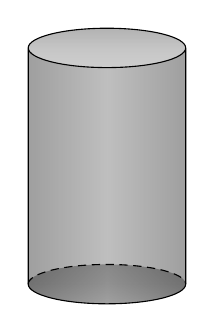
\begin{tikzpicture}[scale=0.5]
      \fill[top color=gray!50!black,bottom color=gray!10,middle color=gray,shading=axis,opacity=0.25] (0,0) circle (2cm and 0.5cm);
      \fill[left color=gray!50!black,right color=gray!50!black,middle color=gray!50,shading=axis,opacity=0.25] (2,0) -- (2,6) arc (360:180:2cm and 0.5cm) -- (-2,0) arc (180:360:2cm and 0.5cm);
      \fill[top color=gray!90!,bottom color=gray!2,middle color=gray!30,shading=axis,opacity=0.25] (0,6) circle (2cm and 0.5cm);
      \draw (-2,6) -- (-2,0) arc (180:360:2cm and 0.5cm) -- (2,6) ++ (-2,0) circle (2cm and 0.5cm);
      \draw [densely dashed] (-2,0) arc (180:0:2cm and 0.5cm);
    \end{tikzpicture}
  \end{center}
  \begin{center}
    \begin{tikzpicture}[>={Stealth[width=2mm,length=3mm]}]
      \fill[color=gray!20] (0,0) circle(3);
      \fill[color=gray!50] (0,0) circle(2.2);
      \fill[color=gray!20] (0,0) circle(2.0);
      \draw [-{Latex[length=2mm]}] (-4,0) -- (4,0) node [above left]  {$X$};
      \draw [-{Latex[length=2mm]}] (0,-4) -- (0,4) node [below right] {$Y$};
      \draw [color=black, line width=1pt] (0,0) circle (3);
      \draw [color=black, line width=1pt,dashed] (0,0) circle (2);
      \draw [color=black, line width=1pt,dashed] (0,0) circle (2.2);
      \draw [->] (0,0)--(1.414,1.414) node[pos=0.5, above] {$r$};
    \end{tikzpicture}
  \end{center}
  By definition, the moment of inertia is

  \begin{equation*}
    I_{\text{cylinder},z}=\int_{V}\rho(x^{2}+y^{2})dV
  \end{equation*}
  The volume of a cylinder is given by

  \begin{equation*}
    V=\pi r^{2}L
  \end{equation*}
  A differential volume element is given by

  \begin{equation*}
    dV=2\pi rLdr
  \end{equation*}
  where $r^{2}=x^{2}+y^{2}$.
  Substituting this into the expression for moment of inertia

  \begin{equation*}
    \begin{split}
      I_{\text{cylinder}}
      &=\int_{0}^{R}\rho r^{2}2\pi rLdr \\
      &=2\pi L\rho\int_{0}^{R}r^{3}dr \\
    \end{split}
  \end{equation*}
  \begin{equation*}
    \begin{split}
      I_{\text{cylinder}}&=\frac{\pi L\rho R^{4}}{2}
    \end{split}
  \end{equation*}
  But, for a cylinder, $M=\rho V=\rho\phi R^{2}L$ giving

  \begin{empheq}[box=\roomyfbox]{equation*}
    I_{\text{cylinder}}=\frac{1}{2}MR^{2}
  \end{empheq}
\end{example}

\begin{example}[Rectangular Cube]
  \begin{center}
    \begin{tikzpicture}[>={Stealth[width=2mm,length=3mm]}]
      \fill[color=gray!20] (0,0) (-4,-3)rectangle(4,3);
      \fill[color=gray!50] (2,2) (1.8,1.8)rectangle(2.2,2.2);
      \draw [color=black, line width=1pt] (0,0) (-4,-3)rectangle(4,3);
      \draw [color=black, line width=1pt,dashed] (2,2) (1.8,1.8)rectangle(2.2,2.2);
      \draw [-{Latex[length=2mm]}] (-5,0) -- (5,0) node [above left]  {$X$};
      \draw [-{Latex[length=2mm]}] (0,-4) -- (0,4) node [below right] {$Y$};
      \draw [->] (0,0)--(2,2) node[pos=0.5, below] {$r$};
      \draw [->] (0,0)--(2,0) node[pos=0.5, below] {$x$};
      \draw [->] (0,0)--(0,2) node[pos=0.5, left] {$y$};
      \draw [color=gray] (0,2)--(2,2);
      \draw [color=gray] (2,0)--(2,2);
      \draw (0,3) node [above left]  {$l$};
      \draw (4,0) node [below right]  {$h$};
    \end{tikzpicture}
  \end{center}
  This cube has depth $w$ into the page.
  $z$ axis is coming out of the page.
  By definition, the moment of inertia is

  \begin{equation*}
    I_{\text{cube},z}=\int_{V}\rho (x^{2}+y^{2})dV
  \end{equation*}
  The volume of a cube is given by

  \begin{equation*}
    V=wxy
  \end{equation*}
  A differential volume element is given by

  \begin{equation*}
    dV=wdxdy
  \end{equation*}
  Substituting this into the expression for moment of inertia

  \begin{equation*}
    I_{\text{cube},z}=\int_{-\frac{l}{2}}^{\frac{l}{2}}\int_{-\frac{h}{2}}^{\frac{h}{2}}\rho(x^{2}+y^{2})wdxdy
  \end{equation*}

  \begin{equation*}
    \begin{split}
      I_{\text{cube},z}&=\rho w\left[\int_{-\frac{h}{2}}^{\frac{h}{2}}(yx^{2}+\frac{y^{3}}{3})dx\right]_{y=-\frac{l}{2}}^{y=\frac{l}{2}} \\
      &=\rho w\int_{-\frac{h}{2}}^{\frac{h}{2}}\left(\frac{l}{2}x^{2}+\frac{l^{3}}{24}\right)-\left(-\frac{l}{2}x^{2}-\frac{l^{3}}{24}\right)dx \\
      &=\rho w\int_{-\frac{h}{2}}^{\frac{h}{2}}lx^{2}+\frac{l^{3}}{12}dx \\
      &=\rho w\left[\frac{l}{3}x^{3}+\frac{l^{3}}{12}x\right]_{x=-\frac{h}{2}}^{x=\frac{h}{2}} \\
      &=\rho w\left[\left(\frac{lh^{3}}{24}+\frac{hl^{3}}{24}\right)-\left(-\frac{lh^{3}}{24}-\frac{hl^{3}}{24}\right)\right]_{x=-\frac{h}{2}}^{x=\frac{h}{2}} \\
      &=\rho w\left(\frac{lh^{3}}{12}+\frac{hl^{3}}{12}\right) \\
      &=\rho wlh\left(\frac{h^{2}+l^{2}}{12}\right) \\
    \end{split}
  \end{equation*}

  \begin{empheq}[box=\roomyfbox]{equation*}
    I_{\text{cube},z}=m\frac{h^{2}+l^{2}}{12}
  \end{empheq}
\end{example}

\begin{example}[Sphere]
  \begin{equation*}
    V_{\text{sphere}}=\frac{4}{3}\pi r^{3}
  \end{equation*}
\end{example}

\begin{example}[Cone]
  \begin{center}
    \begin{tikzpicture}[>={Latex[length=2mm]}]
      \fill[top color=gray!50!black,bottom color=gray!10,middle color=gray,shading=axis,opacity=0.25] (0,0) circle (2cm and 0.5cm);
      \fill[left color=gray!50!black,right color=gray!50!black,middle color=gray!50,shading=axis,opacity=0.25] (2,0) -- (0,6) -- (-2,0) arc (180:360:2cm and 0.5cm);
      \draw (-2,0) arc (180:360:2cm and 0.5cm) -- (0,6) -- cycle;
      \draw [densely dashed] (-2,0) arc (180:0:2cm and 0.5cm);
      \draw [->] (-3,0) -- (3,0) node [above left]  {$Y$};
      \draw [->] (0,-1) -- (0,7) node [below right] {$Z$};
      \draw [->] (2,1) -- (-2,-1) node [below right] {$X$};
    \end{tikzpicture}
  \end{center}
  Find the centroid.
  The cone is symmetric about the $z$ axis, so the centroid is along the $z$ axis, and we just need to find where.

  \begin{equation*}
    z_{cm}=\frac{\int_{m}zdm}{\int_{m}dm}
  \end{equation*}
  Since the cone has constant density we have that $dm=\rho dV$ and so this equation becomes the following, where the constant density is pulled out of the integral and cancels

  \begin{equation*}
    z_{cm}=\frac{\int_{V}zdV}{\int_{V}dV}
  \end{equation*}
  We integrate over this volume by using a stack of thin disks, and integrating from $z=0$ to $z=h$.
  Each disk has radius $r$.
  We find the formula for the disk radius with $z$ as

  \begin{equation*}
    r=R-\frac{R}{h}z
  \end{equation*}
  A differential volume element is given by

  \begin{equation*}
    \begin{split}
      dV&=\pi r^{2}dz \\
      &=\pi\left(R-\frac{R}{h}z\right)^{2}dz \\
      &=\pi R\left(1-\frac{1}{h}z\right)^{2}dz \\
      &=\pi R\left(1-\frac{2z}{h}+\frac{z^{2}}{h^{2}}\right)dz
    \end{split}
  \end{equation*}
  integrating
\end{example}

\begin{empheq}[box=\fboxTwo]{alignat*=3}
  &\mbox{\textbf{Cylinder radius $r$:}} &\hspace{0.5in} I_{\text{cylinder}}=\frac{1}{2}mr^{2} \\
  &\mbox{\textbf{Sphere radius $r$:}} &\hspace{0.5in} I_{\text{sphere}}=\frac{2}{5}mr^{2} \\
  &\mbox{\textbf{Rod length $L$ about end:}} &\hspace{0.5in} I_{\text{rod,end}}=\frac{1}{3}mL^{2} \\
  &\mbox{\textbf{Rod length $L$ about center:}} &\hspace{0.5in} I_{\text{rod,center}}=\frac{1}{12}mL^{2} \\
\end{empheq}

% % TODO@dpwiese - need this def here? Move it to preamble?
% \def\sc{1.6cm}

% \begin{tikzpicture} [x=\sc, y=\sc, line width = 1.5, >=angle 45 ]
%   % axes
%   \draw [line width=1, ->] (-.5,0) -- (2,0) node [right] {$x$};
%   \draw [line width=1, ->] (0,-.5) -- (0,2.3) node [above] {$y$};
%   % triangle
%   \draw (0,0) -- (1,0) -- (1,1.732) -- cycle;
%   % little element
%   \draw (.65,.5) coordinate (a) rectangle ++(.2,.2);
%   \draw [line width=1, gray] (0,0) -- (a) node [pos=.5,right, black] {$r$};
%   % ticks and labels
%   \draw [line width=1] (1,0) -- ++(0,-1ex) node [below] {$1$};
%   \draw [line width=1] (0,1.732) -- ++(-1ex,0) node [left] {$\sqrt3$};
%   \node at (1,.8) [right] {$r=\sec\theta$};
% \end{tikzpicture}

\chapter{Lagrange}

Holonomic system: the number of independent coordinates in the large is equal to the number of independent admissible variations.
Non-holonomic system is not holonomic.
Usually the number of admissible variations are less than the number of generalized coordinates.
Usually we can see nonholonomic systems by allowing the system to undergo large motions.
Remember example of coin rolling without slipping on table.

\begin{enumerate}
  \item{choose generalized coordinates in the large $\xi_{1},\dots,\xi_{n}$}
  \begin{itemize}
    \item{A complete set of coordinates should be able to exactly define the orientation of the system without ambiguity}
    \item{%
      An independent set of coordinates should not have any redundancy.
      In other words, none of the generalized coordinates should be able to be written in terms of the others.
      Should be the minimal amount of coordinates that can describe the orientation of the system
    }
  \end{itemize}
  \item{%
    Consider displacement about each of these coordinates one at a time, while holding all the others fixed.
    Calculate the incremental work $\delta W$ done by the external forces under the incremental displacement $\delta\xi_{j}$.
    Express this incremental work as $\delta W=\Xi_{j}\delta\xi_{j}$ to see what the generalized force is.
    Repeat this for each of the generalized coordinates.
  }
  \item{Find kinetic and potential energy $T$ and $V$ for the system.}
  \item{Make lagrangian $\mathscr{L}=T-V$}
  \item{Use the formula}
  \begin{equation*}
    \frac{d}{dt}\left(\frac{\partial\mathscr{L}}{\partial\dot{\xi}_{j}}\right)-\frac{\partial\mathscr{L}}{\partial\xi_{j}}=\Xi_{j}
  \end{equation*}
  That gives us the equations of motion
\end{enumerate}

\chapter{Problems}

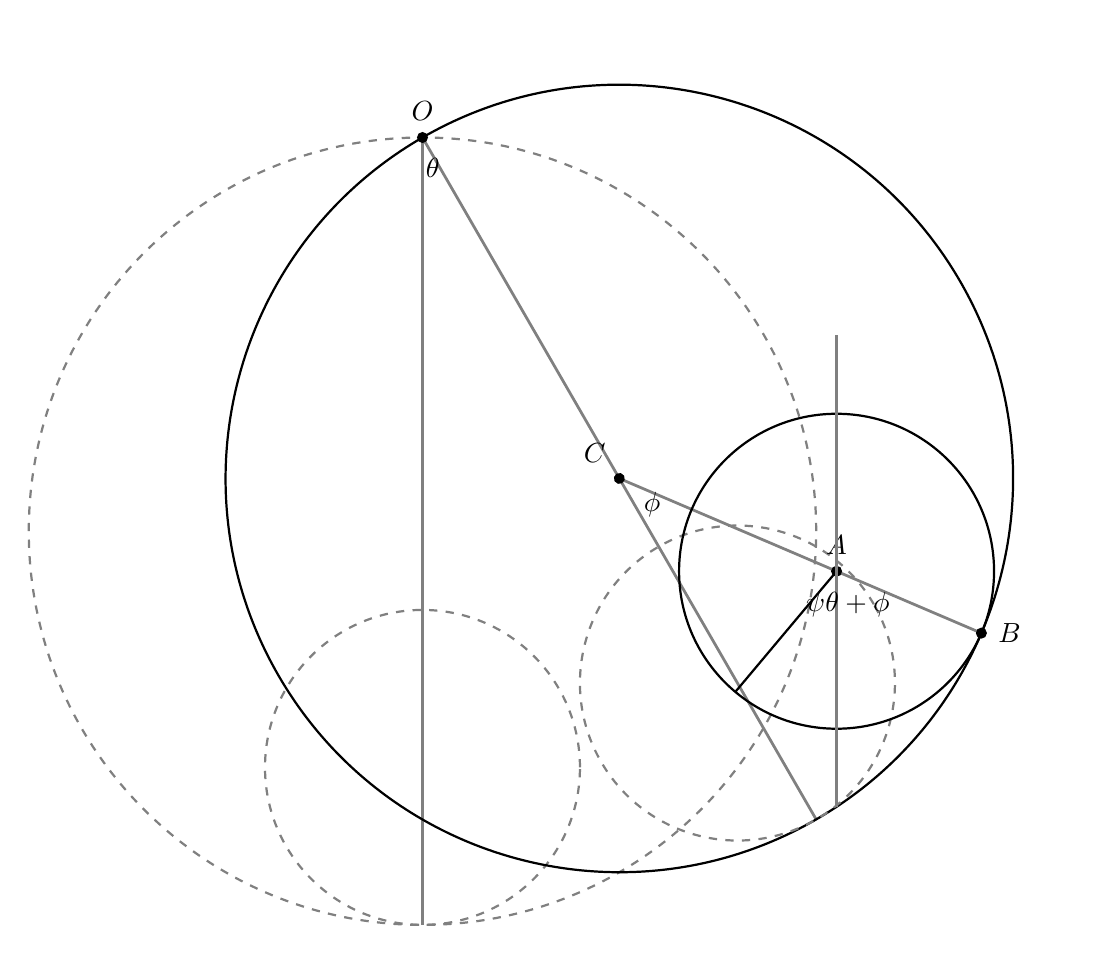
\begin{tikzpicture}[thick]
  %Original, undisplaced configuration
  \draw [color=gray, dashed] circle(5cm);
  \draw [color=gray, dashed] (0,-3) circle(2cm);
  \draw [color=gray, line width=1] (0,5) -- (0,-5);
  % Rotation about theta only, cylinder "glued" to ring
  \draw [color=gray, line width=1, rotate around={30:(0,5)}] (0,5) -- (0,-5) node[pos=0, name=O]{};
  \draw [rotate around={30:(0,5)}] circle(5cm);
  \draw [color=gray, dashed, rotate around={30:(0,5)}] (0,-3) circle(2cm);
  \draw [color=gray, line width=1, rotate around={30:(0,5)}] (0,0) -- (3,-4) node[pos=0.6, name=A]{} node[pos=1.0, name=B]{};
  \node  at (A) [draw,circle,minimum width=4cm] {};
  \node [circle, fill=black, inner sep=0pt,minimum size=4pt, label=$C$,rotate around={30:(0,5)}, name=C] (0,-5) {};
  \node at (O) [circle, fill=black, inner sep=0pt, minimum size=4pt, label=$O$] {};
  \node at (A) [circle, fill=black, inner sep=0pt, minimum size=4pt, label=$A$] {};
  \node at (B) [circle, fill=black, inner sep=0pt, minimum size=4pt, label=right:$B$] {};
  \node at (O) [label=below:$\theta$, anchor=west] {};
  \node [label=below:$\phi$, anchor=west, rotate around={30:(0,5)}] (0,-5){};
  \draw (A.center) --++ (230:2cm);
  \draw [color=gray] (A.center) --++ (0,3) --++ (0,-6);
  \node at (A.east) [label=below:$\theta+\phi$, anchor=west] {};
  \node at (A.west) [label=below:$\psi$, anchor=east] {};
\end{tikzpicture}

Looking at the arc lengths, and how the cylinder rolled inside the ring, with $\psi$ the absolute angular displacement of the cylinder, we have

\begin{equation*}
  \begin{split}
    (\psi+\theta+\phi)r&=\phi R \\
    \psi&=\frac{\phi(R-r)-\theta r}{r} \\
    \psi&=\phi\left(\frac{R}{r}-1\right)-\theta
  \end{split}
\end{equation*}

and so differentiating to get the angular velocity of the cylinder

\begin{equation*}
  \dot{\psi}=\dot{\phi}\left(\frac{R}{r}-1\right)-\dot{\theta}
\end{equation*}

But we can also find this relationship using first principles: equations for motions of rigid bodies.
Since there is no slip, we will find expressions for the velocity of the material point of the ring where it touches the cylinder (point $B$) and do the same for the material point of the cylinder where it touches the ring (again point $B$).
By equating these two expressions, we should be able to solve for $\dot{\psi}$ in terms of the two generalized coordinates $\theta$ and $\phi$ and their derivatives and constants.

\begin{equation*}
  \underline{v}_{B}\bigr|_{\text{ring}}=\underline{\omega}_{\text{ring}}\times\underline{r}_{OB}
\end{equation*}

\begin{empheq}[box=\roomyfbox]{equation*}
  \underline{\omega}_{\text{ring}}=\dot{\theta}\underline{\hat{e}}_{Z}
\end{empheq}

\begin{equation*}
  \underline{r}_{OB}=\underline{r}_{OC}+\underline{r}_{CB}
\end{equation*}

\begin{equation*}
  \underline{r}_{OC}=R\sin\theta\underline{\hat{e}}_{X}-R\cos\theta\underline{\hat{e}}_{Y}
\end{equation*}

\begin{equation*}
  \underline{r}_{CB}=R\sin(\theta+\phi)\underline{\hat{e}}_{X}-R\cos(\theta+\phi)\underline{\hat{e}}_{Y}
\end{equation*}

\begin{equation*}
  \underline{v}_{B}\bigr|_{\text{ring}}=\dot{\theta}R(\sin\theta+\sin(\theta+\phi))\underline{\hat{e}}_{Y}+\dot{\theta}R(\cos\theta+\cos(\theta+\phi))\underline{\hat{e}}_{X}
\end{equation*}

\begin{equation*}
  \underline{v}_{B}\bigr|_{\text{disk}}=\underline{v}_{A}+\underline{\omega}_{\text{disk}}\times\underline{r}_{AB}
\end{equation*}

\begin{equation*}
  \underline{v}_{A}=\underline{v}_{C}+(\dot{\theta}+\dot{\phi})\underline{\hat{e}}_{Z}\times\underline{r}_{OC}
\end{equation*}

\begin{equation*}
  \underline{v}_{C}=\dot{\theta}\underline{\hat{e}}_{Z}\times\underline{r}_{OC}
\end{equation*}

\begin{empheq}[box=\roomyfbox]{equation*}
  \underline{v}_{C}=\dot{\theta}R\sin\theta\underline{\hat{e}}_{Y}+\dot{\theta}R\cos\theta\underline{\hat{e}}_{X}
\end{empheq}

\begin{equation*}
  \underline{r}_{CA}=(R-r)\sin(\theta+\phi)\underline{\hat{e}}_{X}-(R-r)\cos(\theta+\phi)\underline{\hat{e}}_{Y}
\end{equation*}

\begin{equation*}
  \underline{v}_{A}=\dot{\theta}R\cos\theta\underline{\hat{e}}_{X}+\dot{\theta}R\sin\theta\underline{\hat{e}}_{Y}+(\dot{\theta}+\dot{\phi})(R-r)\sin(\theta+\phi)\underline{\hat{e}}_{Y}+(\dot{\theta}+\dot{\phi})(R-r)\cos(\theta+\phi)\underline{\hat{e}}_{X}
\end{equation*}

\begin{empheq}[box=\roomyfbox]{equation*}
  \underline{v}_{A}=\bigr(\dot{\theta}R\cos\theta+(\dot{\theta}+\dot{\phi})(R-r)\cos(\theta+\phi)\bigr)\underline{\hat{e}}_{X}+\bigr(\dot{\theta}R\sin\theta+(\dot{\theta}+\dot{\phi})(R-r)\sin(\theta+\phi)\bigr)\underline{\hat{e}}_{Y}
\end{empheq}

\begin{equation*}
  \underline{v}_{B}\bigr|_{\text{disk}}=\underline{v}_{A}-\omega_{\text{disk}}\underline{\hat{e}}_{Z}\times(r\sin(\theta+\phi)\underline{\hat{e}}_{X}-r\cos(\theta+\phi)\underline{\hat{e}}_{Y})
\end{equation*}
Equating the two velocities of disk and ring, and separating into $X$ and $Y$ components we have

\begin{equation*}
  \begin{split}
    \dot{\theta}R\cos\theta+\dot{\theta}R\cos(\theta+\phi)&=\dot{\theta}R\cos\theta+(\dot{\theta}+\dot{\phi})(R-r)\cos(\theta+\phi)-\omega_{\text{disk}}r\cos(\theta+\phi) \\
    \dot{\theta}R(\sin\theta+\sin(\theta+\phi))&=\dot{\theta}R\sin\theta+(\dot{\theta}+\dot{\phi})(R-r)\sin(\theta+\phi)=\omega_{\text{disk}}r\sin(\theta+\phi)
  \end{split}
\end{equation*}
and both these equations simplify to

\begin{equation*}
  \dot{\theta}R=(\dot{\theta}+\dot{\phi})(R-r)-\omega_{\text{disk}}r
\end{equation*}
giving

\begin{equation*}
  \omega_{\text{disk}}=\dot{\phi}\left(\frac{R}{r}-1\right)-\dot{\theta}
\end{equation*}

\begin{empheq}[box=\roomyfbox]{equation*}
  \underline{\omega}_{\text{disk}}=\left\{\dot{\phi}\left(\frac{R}{r}-1\right)-\dot{\theta}\right\}\underline{\hat{e}}_{Z}
\end{empheq}
Now start doing Lagrangian stuff.
Start by writing an expression for the kinetic energy $T$ and potential energy $V$.

\begin{equation*}
  I_{\text{ring}}=MR^{2}
\end{equation*}

\begin{equation*}
  I_{\text{disk}}=\frac{1}{2}mr^{2}
\end{equation*}

\begin{empheq}[box=\roomyfbox]{equation*}
  V=-MgR\cos\theta-mg(R\cos\theta+\cos(\theta+\phi)(R-r))
\end{empheq}

\begin{equation*}
  T=\frac{1}{2}M\underline{v}_{C}\cdot\underline{v}_{C}+\frac{1}{2}I_{\text{ring}}\omega_{\text{ring}}^{2}+\frac{1}{2}m\underline{v}_{A}\cdot\underline{v}_{A}+\frac{1}{2}I_{\text{disk}}\omega_{\text{disk}}^{2}
\end{equation*}

\begin{equation*}
  \begin{split}
    \underline{v}_{C}\cdot\underline{v}_{C}
    &=(\dot{\theta}R\sin\theta)^{2}+(\dot{\theta}R\cos\theta)^{2} \\
    &=\dot{\theta}^{2}R^{2}
  \end{split}
\end{equation*}

\begin{equation*}
  \omega_{\text{ring}}^{2}=\dot{\theta}^{2}
\end{equation*}

\begin{equation*}
  \begin{split}
    \underline{v}_{A}\cdot\underline{v}_{A}
    &= (\dot{\theta}R\cos\theta+(\dot{\theta}+\dot{\phi})(R-r)\cos(\theta+\phi))^{2} \\
    &+ (\dot{\theta}R\sin\theta+(\dot{\theta}+\dot{\phi})(R-r)\sin(\theta+\phi))^{2}
  \end{split}
\end{equation*}

\begin{equation*}
  \begin{split}
    \underline{v}_{A}\cdot\underline{v}_{A}
    &= \dot{\theta}^{2}R^{2}\cos^{2}\theta+2\dot{\theta}R\cos\theta(\dot{\theta} \\
    &+ \dot{\phi})(R-r)\cos(\theta+\phi)+(\dot{\theta}+\dot{\phi})^{2}(R-r)^{2}\cos^{2}(\theta+\phi) \\
    &+ \dot{\theta}^{2}R^{2}\sin^{2}\theta+2\dot{\theta}R\sin\theta(\dot{\theta}+\dot{\phi})(R-r)\sin(\theta+\phi) \\
    &+ (\dot{\theta}+\dot{\phi})^{2}(R-r)^{2}\sin^{2}(\theta+\phi)
  \end{split}
\end{equation*}

\begin{equation*}
  \begin{split}
    \underline{v}_{A}\cdot\underline{v}_{A}
    &= \dot{\theta}^{2}R^{2}+(\dot{\theta}+\dot{\phi})^{2}(R-r)^{2} \\
    &+ 2\dot{\theta}R\cos\theta(\dot{\theta}+\dot{\phi})(R-r)\cos(\theta+\phi) \\
    &+ 2\dot{\theta}R\sin\theta(\dot{\theta}+\dot{\phi})(R-r)\sin(\theta+\phi)
  \end{split}
\end{equation*}

\begin{equation*}
  \begin{split}
    \underline{v}_{A}\cdot\underline{v}_{A}
    &= \dot{\theta}^{2}R^{2}+(\dot{\theta}+\dot{\phi})^{2}(R-r)^{2} \\
    &+ 2\dot{\theta}R(\dot{\theta}+\dot{\phi})(R-r)\bigr(\cos\theta\cos(\theta+\phi)+\sin\theta\sin(\theta+\phi)\bigr)
  \end{split}
\end{equation*}

\begin{equation*}
  \cos\theta\cos(\theta+\phi)+\sin\theta+\sin(\theta+\phi)=\cos(-\phi)=\cos\phi
\end{equation*}

\begin{equation*}
  \underline{v}_{A}\cdot\underline{v}_{A}
  = \dot{\theta}^{2}R^{2}+(\dot{\theta}+\dot{\phi})^{2}(R-r)^{2}+2\dot{\theta}R(\dot{\theta}+\dot{\phi})(R-r)\cos\phi
\end{equation*}

\begin{equation*}
  \omega_{\text{disk}}^{2}=\left\{\dot{\phi}\left(\frac{R}{r}-1\right)-\dot{\theta}\right\}^{2}
\end{equation*}

\begin{equation*}
  \begin{split}
    T
    &= \frac{1}{2}M\dot{\theta}^{2}R^{2}+\frac{1}{2}MR^{2}\dot{\theta}^{2} \\
    &+ \frac{1}{2}m\left(\dot{\theta}^{2}R^{2}+(\dot{\theta}+\dot{\phi})^{2}(R-r)^{2} + 2\dot{\theta}R(\dot{\theta}+\dot{\phi})(R-r)\cos\phi\right) \\
    &+ \frac{1}{4}mr^{2}\left\{\dot{\phi}\left(\frac{R}{r}-1\right)-\dot{\theta}\right\}^{2}
  \end{split}
\end{equation*}

\begin{empheq}{alignat*=3}
  T
  &= M\dot{\theta}^{2}R^{2} \\
  &\qquad+\frac{1}{2}m\Bigl(\dot{\theta}^{2}R^{2}
  + (\dot{\theta}+\dot{\phi})^{2}(R-r)^{2}+2\dot{\theta}R(\dot{\theta}
  + \dot{\phi})(R-r)\cos\phi\Bigr) \\
  &\qquad+\frac{1}{4}mr^{2}\left\{\dot{\phi}\left(\frac{R}{r}-1\right)-\dot{\theta}\right\}^{2}
\end{empheq}

\begin{empheq}[box=\roomyfbox]{alignat*=3}
  T
  &= M\dot{\theta}^{2}R^{2}+\frac{1}{2}m\dot{\theta}^{2}R^{2} \\
  &\qquad+ \frac{1}{2}m(\dot{\theta}^{2}+2\dot{\phi}\dot{\theta}+\dot{\phi}^{2})(R-r)^{2} \\
  &\qquad+ mR(\dot{\theta}^{2}+\dot{\phi}\dot{\theta})(R-r)\cos\phi{} \\
  &\qquad+ \frac{1}{4}mr^{2}\left\{\dot{\phi}\left(\frac{R}{r}-1\right)-\dot{\theta}\right\}^{2}
\end{empheq}

\begin{equation*}
  V=-MgR\cos\theta-mg(R\cos\theta+\cos(\theta+\phi)(R-r))
\end{equation*}

\begin{equation*}
  \mathscr{L}=T-V
\end{equation*}

\begin{equation*}
  \begin{split}
    \frac{\partial\mathscr{L}}{\partial\dot{\theta}}
    &= 2M\dot{\theta}R^{2}+m\dot{\theta}R^{2}+m(\dot{\theta}+\dot{\phi})(R-r)^{2} \\
    &+ mR(2\dot{\theta}+\dot{\phi})(R-r)\cos\phi+\frac{1}{2}mr^{2}\left\{\dot{\phi}\left(\frac{R}{r}-1\right)-\dot{\theta}\right\}
  \end{split}
\end{equation*}

\begin{equation*}
  \frac{\partial\mathscr{L}}{\partial\theta}=MgR\sin\theta+mgR\sin\theta+mg\sin(\theta+\phi)(R-r)
\end{equation*}

\begin{equation*}
  \frac{\partial\mathscr{L}}{\partial\dot{\phi}}=m(\dot{\theta}+\dot{\phi})(R-r)^{2}+mR\dot{\theta}(R-r)\cos\phi+\frac{1}{2}mr^{2}\left\{\dot{\phi}\left(\frac{R}{r}-1\right)-\dot{\theta}\right\}\left(\frac{R}{r}-1\right)
\end{equation*}

\begin{equation*}
  \frac{\partial\mathscr{L}}{\partial\phi}=
\end{equation*}

\section{Wave Equation on String}

This page gives an outline of the general procedure to derive the equation of motion, propose a general solution, and solve for constants using boundary and initial conditions (here we assume the boundary conditions are both ends fixed, and zero initial conditions just to get the mode shapes and natural frequencies.)

\textbf{Physical assumptions:} \textit{homogenous string $\rho A=\text{constant}$, the string is perfectly elastic (no resistance to bending), the tension is way more than gravity, and string only vibrates perfectly up and down.}

\begin{enumerate}
  \setlength{\itemsep}{0pt}
  \item{\textbf{Derive governing equation}}
  \begin{enumerate}
    \setlength{\itemsep}{0pt}
    \item{Momentum in $x$-direction gives $T(x)$ is constant}
    \item{Do momentum in the $y$-direction}
    \item{Use small angles: $\sin(\alpha+\frac{\partial\alpha}{\partial{}x}dx)=\alpha+\frac{\partial\alpha}{\partial{}x}dx$ and $\tan(\alpha)=\alpha$}
  \end{enumerate}
  The governing equation is $\boxed{T\frac{\partial^{2}y}{\partial{}x^{2}}=\rho A\frac{\partial^{2}y}{\partial{}t^{2}}}$
  \item{\textbf{Propose a general separable solution} $\boxed{y(x,t)=a(x)f(t)}$}
  \begin{enumerate}
    \setlength{\itemsep}{0pt}
    \item{Rearrange the governing equation as $C^{2}\frac{\partial^{2}y}{\partial{}x^{2}}=\frac{\partial^{2}y}{\partial{}t^{2}}$ and propose $f(t)=Ae^{i\omega_{n}t}$ giving $y(x,t)=a(x)Ae^{i\omega_{n}t}$ and plug in}
    \item{The governing equation becomes $C^{2}\frac{\partial^{2}a}{\partial{}x^{2}}+\omega_{n}^{2}a(x)=0$}
    \item{Propose $a(x)=Be^{i\lambda x}$ and get $\omega_{n}=C\lambda$}
    \item{The total solution is then $\boxed{y(x,t)=Be^{i\frac{\omega_{n}}{C} x}Ae^{i\omega_{n}t}}$ which can be decomposed into sine and cosine as $y(x,t)=(B_{1}\sin(\lambda x)+B_{2}\cos(\lambda x))(A_{1}\sin(\omega_{n}t)+A_{2}\cos(\omega_{n}t))$}
  \end{enumerate}
  \item{\textbf{Apply boundary and initial conditions} to get the constants}
  \begin{enumerate}
    \setlength{\itemsep}{0pt}
    \item{%
      Apply boundary conditions $y(x=0,t)=y(x=L,t)=0$ gives $B_{2}=0$ and $B_{1}\sin(\frac{\omega_{n}}{C}L)=0$ so $\frac{\omega_{n}}{C}L=n\pi$ where $n=1,2,3\dots$.
      So $\omega_{n}=\frac{Cn\pi}{L}$.
      The solution becomes $y(x,t)=B_{1}\sin(\frac{\omega_{n}}{C}x)(A_{1}\sin(\omega_{n}t)+A_{2}\cos(\omega_{n}t))$
    }
    \item{Apply initial conditions $y(x,t=0)=0$ gives $A_{2}=0$ reducing solution to $y(x,t)=B_{1}\sin(\frac{\omega_{n}}{C}x) A_{1}\sin(\omega_{n}t)$ or by combining the constants \newline $\boxed{y(x,t)=C_{n}\sin(\frac{\omega_{n}}{C}x)\sin(\omega_{n}t)}$}
  \end{enumerate}
  \item{Now we have the governing equation, now we see if it is \textbf{self-adjoint} if it satisfies the following conditions}
  \begin{enumerate}[(i)]
    \setlength{\itemsep}{0pt}
    \item{$\int u\rho Avdx=\int v\rho Audx$}
    \item{$\int v\left(-T\frac{\partial^{2}}{\partial{}x^{2}}\right)udx=\int u\left(-T\frac{\partial^{2}}{\partial{}x^{2}}\right)vdx$}
  \end{enumerate}
  The first condition is satisfied automatically, since $u$ and $v$ (in our case $a(x)$ and $f(t)$ commute.)
  We show that the second condition holds by doing integration by parts twice.
  \begin{equation*}
    \begin{split}
      &\int_{0}^{L}a_{i}\left(-T\frac{\partial^{2}}{\partial{}x^{2}}\right)a_{j}dx \\
      &= a_{i}\left(-T\frac{\partial}{\partial{}x}(a_{j})\right)\biggr|_{0}^{L}+\int_{0}^{L}T\frac{\partial}{\partial{}x}(a_{j})\frac{da_{i}}{dx}dx
    \end{split}
  \end{equation*}
  one more integration by parts
  \begin{equation*}
    \begin{split}
      &\int_{0}^{L}a_{i}\left(-T\frac{\partial^{2}}{\partial{}x^{2}}\right)a_{j}dx \\
      &=a_{i}\left(-T\frac{\partial}{\partial{}x}(a_{j})\right)\biggr|_{0}^{L}-\left(\frac{da_{i}}{dx}(-Ta_{j})\right)\biggr|_{0}^{L}+\int_{0}^{L}a_{j}\left(-T\frac{\partial^{2}}{\partial{}x^{2}}(a_{i})\right)dx
      \end{split}
  \end{equation*}
  and since we evaluate the first two terms on the right hand side at $x=0$ and $x=L$, the boundary conditions dictate that $a_{i}=a_{j}=0$ here, thus proving the system is \textbf{self-adjoint}.
  \textit{Self-adjointness depends on the boundary conditions.}
  \item{Now we use the self adjoint property to show that the modes are \textbf{orthogonal}, where $a_{j}$ and $a_{i}$ are orthogonal functions if they satisfy}
  \begin{equation*}
    \int_{0}^{L}a_{j}a_{i}dx=0
  \end{equation*}
\end{enumerate}
